\chapter{Το {\en LensKit}}
\label{Chapter4}

\section{Εισαγωγή}

Το {\en LensKit} \cite{Ekstrand:2011:RRR:2043932.2043958} αποτελεί ένα ανοιχτού κώδικα πακέτο λογισμικού για την πραγματοποίηση μελέτης και επαληθεύσιμης έρευνας πάνω σε συστήματα παραγωγής συστάσεων. Αποτελεί μία πλατφόρμα για την ανάπτυξη αλγορίθμων παραγωγής συστάσεων, μέτρησης της επίδοσής τους πάνω σε διαφορετικά σύνολα δεδομένων και σύγκρισης νέων ιδεών με τις τρέχουσες βέλτιστες πρακτικές. \cite{ekstrand_towards_2014}\footnote{Κύρια πηγή του παρόντος κεφαλαίου ειναι το \cite{ekstrand_towards_2014}.} Υλοποιήθηκε από τον {\en Michael D. Ekstrand} και αναπτύχθηκε από ερευνητές στο {\en Texas State University} και στο πανεπιστήμιο της {\en Minnesota}, με συνεισφορά από προγραμματιστές από όλο τον κόσμο.\footnote{\en \url{http://lenskit.org/}} Αποτελείται από περισσότερες από 49Κ γραμμές κώδικα με συνεισφορά από 28 προγραμματιστές. Είναι γραμμένο κυρίως σε {\en Java} (92\%) και ένα σημαντικό μέρος του είναι σε {\en Groovy} (7\%).\footnote{Στατιστικά από \en BlackDuck | Open Hub \url{https://www.openhub.net/p/lenskit}} Ο πηγαίος κώδικας του {\en LensKit} είναι δημοσιευμένος στο {\en GitHub}.\footnote{\en \url{https://github.com/lenskit/lenskit}} Η φιλοσοφία που ακολουθήθηκε για την ανάπτυξη του βασίζεται αρκετά στο \cite{Bloch:2008:EJ:1377533}.\par 
Για το σκοπό που αναπτύχθηκε προσφέρει:
\begin{itemize}
 \item Διεπαφές προγραμματισμού εφαρμογών ({\en APIs}) για την παραγωγή συστάσεων και προβλέψεων. Επιτρέπει στους προγραμματιστές να χρησιμοποιήσουν τους υλοποιημένους αλγόριθμους ως «μαύρο κουτί».
 \item Υλοποίηση βασικών αλγορίθμων για παραγωγή συστάσεων και πρόβλεψη βαθμολογιών. 
 \item Εργαλειοθήκη αξιολόγησης απόδοσης σε κοινά σύνολα δεδομένων με χρήση ποικιλίας μετρικών.
 \item Κώδικα υποστήριξης για την ανάπτυξη νέων αλγορίθμων, μεθόδων αξιολόγησης και άλλων επεκτάσεων.
\end{itemize}
\par Ένας παραγωγός συστάσεων στο {\en LensKit} αποτελείται από ένα σύνολο διεπαφών που παρέχουν παραγωγή συστάσεων και πρόβλεψη βαθμολογιών. Οι διεπαφές αυτές συνδέονται με μία πηγή δεδομένων χρησιμοποιώντας έναν ή περισσότερους αλγορίθμους παραγωγής συστάσεων. Η σύγκριση διαφορετικών αλγορίθμων γίνεται με τη χρήση {\en script} (σεναρίου) αφού δηλωθούν οι πηγές δεδομένων, οι αλγόριθμοι και οι μετρικές βάσει των οποίων συγκρίνονται.
\section{Σχεδιασμός του \en LensKit}
Ο σχεδιασμός του {\en LensKit} έγινε με στόχο τόσο την άναπτυξη και την έρευνα πάνω σε συστήματα παραγωγής συστάσεων όσο και τη χρήση του σε εκπαιδευτικούς σκοπούς. Το πανεπιστήμιο της {\en Minnesota} χρησιμοποιεί το {\en LensKit} τόσο σε μεταπτυχιακό του μάθημα όσο και σε {\en MOOC} πάνω σε συστήματα παραγωγής συστάσεων που προσφέρει μέσω της πλατφόρμας {\en Coursera}. To {\en LensKit} αναπτύχθηκε με τρόπο που να υποστηρίζει τη διεξαγωγή πειραμάτων.\cite{Konstan:2015:TRS:2744768.2728171} \par
Βασική αρχή στο {\en LensKit} είναι η υλοποίηση των αλγορίθμων ως ένα σύνολο σχεδόν ανεξάρτητων τμημάτων. Ένας τυπικός αλγόριθμος παραγωγής συστάσεων χρειάζεται τουλάχιστον δώδεκα διακριτά τμήματα ({\en components}) που επικοινωνούν μεταξύ τους μέσω καλώς ορισμένων διεπαφών. Αυτή η πρακτική διευκολύνει τη συντήρηση και τoν έλεγχο ορθότητας καθενός από τα συστατικά της υλοποίησης. \par
Βασικός στόχος είναι η διασφάλιση της ορθότητας και στη συνέχεια της αποτελεσματικότητας. Στο {\en LensKit} υπάρχουν πολλά αμετάβλητα αντικείμενα ({\en immutable objects}), ώστε να διασφαλίζεται ότι ένα τμήμα δε θα επηρεάζει αρνητικά τη λειτουργικότητα ενός άλλου. \par
Το {\en LensKit} ακολουθεί το μοτίβο στρατηγικής ({\en Strategy Pattern}). Στο μοτίβο αυτό κατά την ανάπτυξη μιας υλοποίησης δε χρησιμοποιείται η κληρονομικότητα. Αντί για υποκλάσεις που θα υλοποιούν τους διαφορετικούς τρόπους που μία κλάση θα επιτελεί κάποια λειτουργία της, χρησιμοποιείται η χρήση ξεχωριστών τμημάτων που ορίζονται από διεπαφές.\cite{Gamma:1995:DPE:186897} Η στρατηγική αυτή έχει ως άμεσο αποτέλεσμα οι επιμέρους αλλαγές στα τμήματα που υλοποιούν τις διεπαφές να μην απαιτούν αλλαγές στις κλάσεις που τα χρησιμοποιούν. Επιπρόσθετα, επιτρέπει την επανάχρηση των τμημάτων αυτών από άλλους αλγορίθμους μειώνοντας τον απαιτούμενο κώδικα για την υλοποίηση ενός αλγορίθμου, αλλά και βοηθώντας τον ερευνητή να επικεντρωθεί μόνο στην αναγκαία υλοποίηση που χρειάζεται για να ελέγξει την υπόθεσή του. \par
Παρά το ότι οι υλοποιημένοι αλγόριθμοι στο {\en LensKit} είναι εξαιρετικά διαμορφώσιμοι, δεν απαιτείται από το χρήστη να εμβαθύνει σε κάθε ξεχωριστό τμήμα, ώστε να τους χρησιμοποιήσει, καθώς όπου είναι δυνατό έχουν οριστεί προεπιλογές. 
\par Τέλος, κατά το σχεδιασμό του έχει γίνει προσπάθεια ελαχιστοποίησης των υποθέσεων που αφορούν στο είδος των δεδομένων που θα θελήσουν να χρησιμοποιήσουν οι χρήστες. Παρόμοια προσπάθεια γίνεται και όσον αφορά την υλοποίηση των ίδιων των αλγορίθμων όσο και του αξιολογητή.
\section{Οργάνωση του κώδικα - Ενότητες}
Ο κώδικας οργανώνεται σε δέκα ενότητες ({\en modules}):
\begin{enumerate}
 \item {\en API}: Περιλαμβάνει τις διεπαφές για υψηλού επιπεδου εργασίες στην παραγωγή συστάσεων. Είναι ανεξάρτητο από τις υπόλοιπες ενότητες εκτός αυτής των δομών δεδομένων.
 \item Δομές Δεδομένων ({\en Data structures}): Περιλαμβάνει τις βασικές δομές δεδομένων του {\en LensKit}.
 \item Πυρήνας ({\en Core}): Περιέχει το κύριο μέρος του {\en LensKit}, εκτός του αξιολογητή και των υλοποιήσεων των αλγορίθμων. Παρέχει υποστήριξη για το χειρισμό δεδομένων και τη διαμόρφωση των αλγορίθμων.
 \item Αξιολογητής ({\en Evaluator}): Περιέχει υποστήριξη για την αξιολόγηση και τη σύγκριση αλγορίθμων με χρήση γνωστών μετρικών.
 \item Παραγωγοί Προβλέψεων ({\en Predictors}): Εξειδικευμένη υποστήριξη για την πρόβλεψη βαθμολογιών.
 \item {\en k-NN}: Συνεργατική Διήθηση πλησιέστερου γείτονα (είδους-είδους και χρήστη-χρήστη).
 \item {\en SVD}: Συνεργατική Διήθηση μέσω παραγοντοποίησης μητρώων. 
 \item {\en Slope1:} Υλοποίηση του αλγορίθμου {\en Slope One}.
 \item {\en Grapht}: Τεχνικά δεν αποτελεί μέρος του. Είναι εργαλειοθήκη της {\en Java} που τη χρησιμοποιεί για το χειρισμό της εισαγωγής εξαρτήσεων ({\en dependency injection}).
 \item {\en CLI:} Διεπαφή γραμμής εντολών για εκτέλεση αλγορίθμων, χειρισμό αρχείων δεδομένων και επιθεώρηση διαμορφώσεων αλγορίθμων.
\end{enumerate}
\begin{figure}[H]
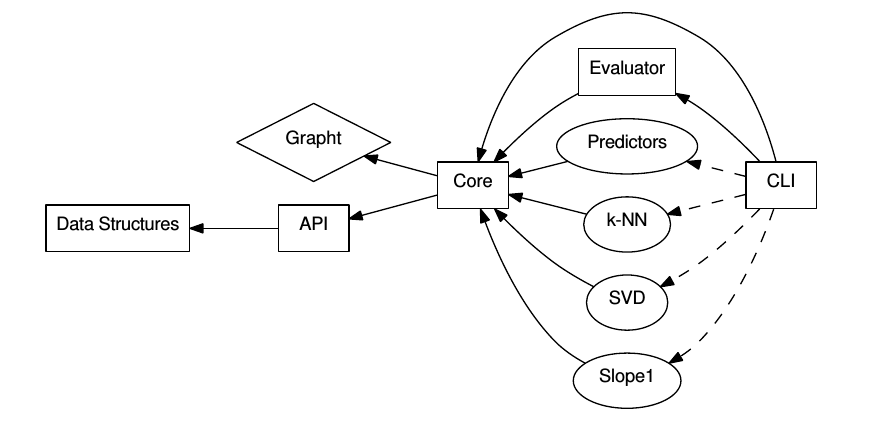
\includegraphics[scale=0.5]{images/st.png}
\caption{Διάγραμμα των ενοτήτων του {\en LensKit} και των μεταξύ τους σχέσεων \cite{ekstrand_towards_2014}}
\end{figure}
\subsection{Διεπαφή Παραγωγών Συστάσεων}
Αποτελεί τη διεπαφή με την οποία το δημόσιο ΑΡΙ είναι προσβάσιμο. Δεν παρέχει υλοποίηση κανενός παραγωγού συστάσεων. Χρησιμοποιείται για την επικοινωνία με τις διεπαφές των διαφόρων τμημάτων που υλοποιούν έναν παραγωγό συστάσεων και για την παροχή πρόσβασης σε εφαρμογές προς αυτά. Είναι διαχωρισμένο από τις υλοποιήσεις των παραγωγών συστάσεων και ανήκει στο δημόσιο ΑΡΙ. \par 
Κεντρικό τμήμα ενός παραγωγού συστάσεων είναι η υλοποίηση της διεπαφής του βαθμολογητή ειδών ({\en Item Scorer}). Ο βαθμολογητής ειδών αποτελεί  γενίκευση της παραγωγής προβλέψεων και υπολογίζει προσωποποιημένες ως προς το χρήστη βαθμολογίες ({\en ratings}). Υπολογίζει τις βαθμολογίες των ειδών ({\en scores}) προβλέπο\-ντας τις βαθμολογίες των χρηστών για αυτά. Αυτό αποτελεί μια γενίκευση που επιτρέπει τη βαθμολογία ειδών ακόμα και από τις εκδηλώσεις προτίμησης των χρηστών. Ο βαθμολογητής ειδών χρησιμοποιείται έμμεσα ενώ άμεσα χρήσιμοποιούνται οι παραγωγοι συστάσεων ειδών και οι παραγωγοί προβλέψεων βαθμολογιών. Και οι τρεις έχουν την ίδια διεπαφή και αυτό που τους διαφοροποιεί είναι ότι οι τελευταίοι αναλαμβάνουν να διεκπεραιώσουν δευτερεύουσες εργασίες που απαιτούνται για την παραγωγή συστάσεων (όπως την αντιστοίχιση των βαθμολογιών σε κάποιο εύρος), ώστε να κρατείται «καθαρός» ο κώδικας του βαθμολογητή και να αποφεύγεται η επικάλυψη κώδικα. 
\section{Μοντέλο Δεδομένων}
Το μοντέλο δεδομένων του {\en LensKit} στοχεύει στην αναπαράσταση και στην πρόσβαση στα δεδομένα που απαιτεί ένας παραγωγός συστάσεων. Για το σκοπό αυτό χρησιμοποιεί τις έννοιες χρήστες ({\en users}), είδη ({\en items}) και γεγονότα ({\en events}). Το μοντέλο αυτό είναι αρκετά ευέλικτο, ώστε να υποστηρίζει και άμεσες βαθμολογίες και έμμεση εκδήλωση προτίμησης. \par
Οι χρήστες και τα είδη αναπαριστώνται με αριθμητικά αναγνωριστικά ({\en numerical identifiers (Java longs)}. \par
Ως γεγονός ορίζεται η αλληλεπίδραση του χρήστη με κάποιο είδος. Για κάθε τύπο γεγονότος, ορίζεται διαφορετική διεπαφή (επεκτάση του βασικού τύπου). Μέχρι στιγμής έχουν υλοποιηθεί τρεις τύποι γεγονότων: η Βαθμολόγηση ({\en Rating})\footnote{\en \url{http://lenskit.org/apidocs/org/grouplens/lenskit/data/event/Rating.html}}, η Προτίμηση ({\en Like})\footnote{\en \url{http://lenskit.org/apidocs/org/grouplens/lenskit/data/event/Like.html}} και η Μαζική Προτίμηση ({\en LikeBatch})\footnote{\en \url{http://lenskit.org/apidocs/org/grouplens/lenskit/data/event/LikeBatch.html}}. Η Προτίμηση χρησιμοποιείται ως έκφραση απλής εκδήλωσης προτίμησης. Η Μαζική Προτίμηση αφορά τις Προτιμήσεις πολλών χρηστών. \par
Η επικοινωνία των διαφόρων τμημάτων του παραγωγού συστάσεων με τα δεδομένα γίνεται μεσω αντικειμένων για πρόσβαση σε δεδομένα ({\en Data Access Objects (DAOs))}. Υπάρχει ευελιξία όσον αφορά τον τρόπο που μπορεί να είναι αποθηκευμένα τα δεδομένα καθώς μπορούν να υλοποιηθούν {\en DAOs} ανάλογα με τις ανάγκες του παραγωγού συστάσεων. Το {\en LensKit} παρέχει {\en DAOs} για χειρισμό αρχείων κειμένου και βάσεων δεδομένων. Έχουν υλοποιηθεί βασικές μέθοδοι, οι οποίες επιστρέφουν βασικές δομές δεδομένων της {\en Java} και μέθοδοι συνεχούς ροής ({\en streaming}) μέθοδοι, οι οποίες επιστρέφουν κέρσορες ({\en cursors}). Οι μέθοδοι συνεχούς ροής προσφέρουν αποδοτική διαχείριση μνήμης καθώς επιτρέπουν την επεξεργασία ενός αντικειμένου κάθε φορά χωρίς να φορτώνονται όλα τα απαιτούμενα αντικείμενα στη μνήμη. Υπάρχει η δυνατότητα επέκτασης των διεπαφών για αξιοποίηση μεταδεδομένων των χρηστών ή των αντικειμένων. Για το {\en LensKit} τα \en DAOs \el είναι τμήματα, όπως αυτά που επιτελούν τις λειτουργίες ενός παραγωγού συστάσεων.
\subsection{Δομές Δεδομένων}
Για την επεξεργασία των δεδομένων είναι συχνά αναγκαία η χρήση διανυσμάτων ({\en vectors}). Για το σκοπό αυτό το {\en LensKit} προσφέρει τα \en Sparse Vectors \el(Αραιά Διανύσματα). Αποτελούν αντιστοίχιση ({\en map}) από {\en long} σε \en double \elκαι είναι αποδοτικά σε πράξεις γραμμικής άλγεβρας. Λειτουργούν ως παράλληλοι πίνακες αναγνωριστικών (\en IDs) \el χρηστών ή ειδών και τιμών και ταξινομούνται βάσει \en ID. \el Ο ορισμός του χώρου κλειδιών τους (\en key domain) \el γίνεται κατά τη στιγμή της δημιουργίας τους και αυτό έχει ως αποτέλεσμα αποδοτική διαχείριση της μνήμης. Τα κλειδιά για τα οποία έχει οριστεί τιμή αποτελούν το σύνολο κλειδιών \en(key set). \el Υπάρχει η αφηρημένη κλάση \en SparseVector \el, η οποία υποστηρίζει μεθοδους μόνο ανάγνωσης. Η κλάση \en ImmutableSparseVector, \el διασφαλίζει τη μη πραγματοποί\-ηση αλλαγών στο διάνυσμα, σε αντίθεση με τη \en MutableSparseVector. \el Αν ο χώρος κλειδιών δεν είναι αρχικά γνωστός γίνεται χρήση πινάκων κατακερματισμού \en (hash map) \el και στη συνέχεια μετατροπή τους σε διανύσματα. \par
Το \en LensKit \el χρησιμοποιεί τη βιβλιοθήκη \en fastutil\footnote{\url{http://fastutil.di.unimi.it/}}\el και το \en Google Guava\footnote{\url{https://github.com/google/guava}}. H fastutil \el παρέχει συλλογές \en (collections), \el οι οποίες είναι συμβατές με τη διεπαφή συλλογών της \en Java (Java Collection API) \el και επιτρέπει στο \en LensKit \el τη χρήση λιστών, συνόλων και αντιστοιχίσεων. Επιπλέον παρέχει γρήγορη επανάληψη (\en fast iteration), \el η οποία μειώνει τις απαιτήσεις δέσμευσης μνήμης. \par
Υπάρχει η πρόθεση αντικατάστασης των \en Sparse Vectors\footnote{\url{https://github.com/lenskit/lenskit/wiki/ReplacingSparseVectors}} \el είτε μέσω των δομών που προσφέρει το \en fastutil \el είτε μέσω αυτών του \en HPPC\footnote{\url{labs.carrotsearch.com/hppc.html}}. \elΕπίσης, υπάρχει η σκέψη δημιουργίας νέων τύπων για τα αποτελέσματα που να υποστηρίζουν την επιστροφή και το χειρισμό περισσότερων πληροφοριών εκτός των συστάσεων, όπως του βαθμού εμπιστοσύνης σε αυτές.\footnote{\en \url{https://github.com/lenskit/lenskit/wiki/DetailedResults}} Στόχος είναι η διατήρηση της αποδοτικότητας, αλλά και η μείωση της πολυπλοκότητας για τους προγραμματιστές.\footnote{\en \url{http://mailman.cs.umn.edu/archives/lenskit/2015q1/000555.html}}
\section{\en Modular \el αλγόριθμοι}
Βασική αρχή σε όλες τις υλοποιήσεις του είναι η τμηματοποίηση των αλγορίθμων, ώστε κάθε τμήμα να εκτελεί μία και μόνο λειτουργία με στόχο την επαναχρησιμοποίηση, την ευκολότερη παραμετροποίηση και την ανάπτυξη κώδικα. Το \en LensKit \el παρέχει τις απαραίτητες υποδομές, ώστε να διευκολύνει την υλοποίηση αλγορίθμων με αυτή τη στρατηγική. \par Το \en LensKit \el χρησιμοποιεί το μοτίβο στρατηγικής \cite{Gamma:1995:DPE:186897}, το οποίο επιτρέπει να υπάρχουν ξεχωριστά τμήματα που επιτελούν λειτουργίες, όπως η κανονικοποίηση δεδομένων τα οποία μπορούν να χρησιμοποιηθούν από τους υλοποιημένους αλγορίθμους. \par
Στο {\en LensKit} γίνεται εκτεταμένη χρήση κατασκευαστών (\en builders)\el. Ακολουθεί\-ται η μέθοδος του διαχωρισμού των τμημάτων που περιέχουν τα δεδομένα (\en data containers) \el (και συνοδεύονται από διεπαφές για την πρόσβαση σε αυτά) και των κατασκευαστών που κάνουν υπολογισμούς για την παραγωγή (φαινομενικά αμετάβλητων) αντικειμένων. Έτσι μπορεί εύκολα να αλλάξει η στρατηγική πραγματοποίησης των απαιτούμενων υπολογισμών χωρίς να αλλάξει η υλοποίηση του υπόλοιπου αλγορίθμου. \par
Επιπλέον χρησιμοποιούν τη τεχνική \en Builder and Facade \el\cite{Gamma:1995:DPE:186897} (Κατασκευή και Εκπροσώπηση), η οποία περιλαμβάνει κατασκευαστές και μία διεπαφή που λειτουργεί ως εκπρόσωπος (διεπαφή) άλλων διεπαφών. \par
Για την επίτευξη των παραπάνω το {\en LensKit} χρησιμοποιεί τη μέθοδο της εισαγωγής εξαρτήσεων \cite{mar96c}, δηλαδή ένα τμήμα κώδικα όταν καλείται πρέπει να του παρέχονται και τα αντικείμενα από τα αποία εξαρτάται αντί αυτά να ενεργοποιού\-νται από το ίδιο το τμήμα. Με την τεχνική αυτή είναι δυνατό να αλλάξει η υλοποίηση κάποιας εξάρτησης και να τροποποιηθεί η συμπεριφορά του εξαρτώμενου τμήματος χωρίς αυτό να επαναπρογραμματιστεί. Για το σκοπό αυτό το {\en LensKit} χρησιμοποιεί την εργαλειοθήκη {\en Grapht}. \par
Τα τμήματα χωρίζονται σε αυτά που είναι προκατασκευασμένα από τα δεδομένα (\en pre-built) \el και μπορούν να χρησιμοποιηθούν από διαφορετικές κλήσεις και αυτά που χρειάζονται άμεση πρόσβαση στα δεδομένα.
\subsection{Βασικές Υλοποιήσεις Τμημάτων}
Λόγω της δομής του \en LensKit \el είναι δυνατόν να υλοποιηθεί κάποιος αλγόριθμος παραγωγής συστάσεων διαμορφώνοντας κάποιον ήδη υλοποιημένο \en item scorer \el ή υλοποιώντας μόνο το κομμάτι του αλγορίθμου που αφορά τον \en item scorer. \el H προεπιλεγμένη υλοποίηση του \en item scorer \el είναι ο \en TopNItemRecommender\footnote{\url{http://lenskit.org/apidocs/org/grouplens/lenskit/basic/TopNItemRecommender.html}},\el ο οποίος χρησιμοποιεί τον \en item scorer \el για να βαθμολογήσει τα είδη και επιστρέφει τα Ν καλύτερα (με προεπιλογή αποκλεισμού των ήδη βαθμολογημένων από τον χρήστη ειδών).\el
\subsection{Παραγωγοί Περιλήψης Ιστορικού και Κανονικοποιητές}
Ένας παραγωγός περιλήψης ιστορικού παράγει από το ιστορικό γεγονότων του χρήστη ένα αραιό διάνυσμα προτιμήσεων του οποίου τα κλειδιά είναι τα είδη και οι τιμές είναι κάποιες πραγματικές τιμές που αντιπροσωπεύουν τις προτιμήσεις του χρήστη. Πολλά συστήματα ενώ δε χρησιμοποιούν άμεσες βαθμολογίες, παράγουν ένα διάνυσμα που σχετίζεται με τις προτιμήσεις του χρήστη. Επίσης αυτό το διάνυσμα συχνά κανονικοποιείται ως προς το μέσο όρο των βαθμολογιών. \par
Οι κανονικοποιητές εφαρμόζονται πάνω σε διανύσματα αναφοράς και διανύσματα στόχους. Το διάνυσμα αναφοράς χρησιμοποιείται για τον υπολογισμό της βάσης της κανονικοποίησης και το διάνυσμα-στόχος είναι αυτό το οποίο τροποποιείται. Για λόγους αντιστρεψιμότητας υπάρχει η δυνατότητα δημιουργίας ενός μετασχηματισμού από ένα διάνυσμα αναφοράς. Ο μετασχηματισμός μετά μπορεί να εφαρμοστεί σε οποιοδήποτε διάνυσμα. Υποστηρίζονται και στοχευμένοι ως προς τον χρήστη ή το αντικείμενο κανονικοποιητές. Οι κανονικοποιητές αυτοί μπορούν να κάνουν χρήση επιπλέον πληροφορίας. Συχνά εξαρτώνται από \en DAOs \el για την πρόσβαση σε δεδομένα ή από κάποιο άλλο τμήμα το οποίο μπορεί να επωφεληθεί απο τη γνώση για το ποιο διάνυσμα κανονικοποιείται.
\subsection{Βαθμολογητές Βάσης}
Υπολογίζουν βαθμολογίες για τα είδη με χρήση απλών μέσων όρων. Χρησιμοποιούνται τόσο σε περίπτωση αποτυχίας του βασικού βαθμολογητή ειδών όσο και για κανονικοποίηση δεδομένων. Βασικοί αλγόριθμοι χρησιμοποιούν κανονικοποιημένα δεδομένα αντί για τις πραγματικές βαθμολογίες. Οι βαθμολογητές βάσης υλοποιούν τη διεπαφή του βαθμολογητή ειδών και οποιοσδήποτε βαθμολογητής ειδών μπορεί να χρησιμοποιηθεί ως βαθμολογητής βάσης. Υποστηρίζουν τη χρήση μιας παραμέτρου απόσβεσης (\en damping parameter)\el, ώστε αντικείμενα με λίγες βαθμολογίες να μην παίρνουν αδικαιολόγητα μεγάλες τιμές. Αν ο χρήστης δεν έχει βαθμολογήσει αρκετά είδη, μπορούν να ανατεθούν οι τιμές του βαθμολογητή βάσης.
\subsection{Διαμόρφωση Αλγορίθμων}
Η διαμόρφωση των αλγορίθμων γίνεται μέσω του \en Grapht API \el με τη χρήση μιας ενσωματωμένης γλώσσας σεναρίων σε \en Groovy, \elη οποία έχει πιo «ελαφριά» σύνταξη σε σχέση με τη \en Java. \el Δίνει τη δυνατότητα οι ορισμοί των αλγορίθμων να αντιμετωπίζονται ως αρχεία διαμόρφωσης ({\en configuration files}) και να μην είναι ενσωματωμένοι στον κώδικα των εφαρμογών. Η γραμμή εντολών του \en LensKit \el μπορεί να χειριστεί αυτά τα σενάρια.
\subsection{Αξιολόγηση Αλγορίθμων και Σύνολα Δεδομένων}
Υποστηρίζεται {\en offline}, προσανατολισμένη στα δεδομένα αξιολόγηση της απόδοσης μέσω εκπαίδευσης και ελέγχου ({\en train/test}) με διαχωρισμό και επαλήθευση ({\en cross-validation}). Υποστηρίζεται επεξεργασία των συνόλων δεδομένων και αξιολόγηση αλγορίθμων πάνω σε πολλαπλά σύνολα δεδομένων και μέτρηση της απόδοσής τους. Στο {\en LensKit 3} θα γίνεται μέσω της διεπαφής γραμμής εντολών ({\en CLI}) και του {\en Gradle}\footnote{\en \url{http://gradle.org/}}.\footnote{\en \url{http://mailman.cs.umn.edu/archives/lenskit/2015q1/000560.html}} Ο αξιολογητής χειρίζεται δεδομένα κυρίως σε μορφή {\en delimited} (οριοθετημένων) αρχείων κειμένου και δυαδικών αρχείων βαθμολογιών. Οι βασικές εργασίες χειρισμού δεδομένων είναι: 
\begin{itemize}
 \item {\en crossfold}: Διαχωρισμός της πηγής δεδομένων σε Ν τμήματα για {\en cross-validation}.
 \item {\en pack}: Μετατροπή ενός συνόλου δεδομένων σε δυαδικό αρχείο για αποδοτική πρόσβαση.
 \item {\en subsample}: Δημιουργία ενός μικρότερου συνόλου δεδομένων με τυχαία επιλογή από ένα μεγαλύτερο βάσει κριτηρίου.\footnote{Θα καταργηθεί στο {\en LensKit 3}.}
\end{itemize}
\subsection{Aξιολόγηση Αλγορίθμων και Mετρικές Απόδοσης}
Ο αξιολογητής δέχεται ένα σύνολο αλγορίθμων και ζεύγη συνόλων δεδομένων εκπαίδευσης και ελέγχου και αξιολογεί την ακρίβεια κάθε αλγορίθμου πάνω σε κάθε ζεύγος. Οι διαθέσιμες μετρικές είναι δύο ειδών\footnote{\en \url{http://lenskit.org/documentation/evaluator/upgrading/}}: μετρικές πρόβλεψης\footnote{\en \url{http://lenskit.org/master/apidocs/org/lenskit/eval/traintest/predict/PredictMetric.html}} και {\en TopN} μετρικές\footnote{\en \url{http://lenskit.org/master/apidocs/org/lenskit/eval/traintest/recommend/TopNMetric.html}}. Οι μετρικές πρόβλεψης περιλαμβάνουν: 
\begin{itemize}
\item {\en MAE}: Μέσο απόλυτο σφάλμα της ακρίβειας των προβλεφθέντων δεδομένων βαθμολόγησης. 
\item {\en RMSE}: Ομοία με μέσο τετραγωνικό σφάλμα. 
\item {\en Coverage \el(κάλυψη)}: Μετράει τον αριθμό των παρεχόμενων προβλέψεων βαθμολογιών και υπολογίζει την κάλυψη σε σχέση με το σύνολο των ζητούμενων.
\item {\en nDCG}: Αξιολογεί τις προβλέψεις του παραγωγού συστάσεων μέσω κανονικοποιημένου μειούμενου συσσωρευτικού οφέλους. Τα είδη ταξινoμούνται βάσει της προβλεφθείσας προτίμησης και η μετρική υπολογίζεται χρησιμοποιώντας τις πραγματικές βαθμολογίες του χρήστη ως συνάρτηση ωφέλειας για κάθε είδος. Με αυτό τον τρόπο δεν «τιμωρεί» τον παραγωγό συστάσεων όταν προτείνει είδη τα οποία θα ήταν καλά για το χρήστη, αλλά για τα οποία δεν είχε δεδομένα.
\end{itemize}
Οι {\en TopN} μετρικές περιλαμβάνουν:
\begin{itemize}
 \item {\en Entropy} (Εντροπία): Εξετάζει το εύρος των προτεινόμενων ειδών σε σχέση με το σύνολο των ειδών για όλους τους χρήστες. Όσο μικρότερη είναι η τιμή που επιστρέφει η μετρική τόσο λιγότερα είναι τα είδη από τα οποία προτείνει ο παραγωγός. Στη χειρότερη περίπτωση τα είδη που προτείνονται είναι τα ίδια για όλους τους χρήστες.
 \item {\en Length} (Μήκος): Υπολογίζει τον αριθμό των συστάσεων. 
 \item {\en MAP}: Υπολογίζει τη μέση ακρίβεια για τους μέσους όρους ακρίβειας κάθε λίστας που επιστρέφεται.
 \item {\en MRR}: Υπολογίζει τη μέση αμοιβαία κατάταξη. 
 \item {\en nDCG}: Όμοια με την αντίστοιχη μετρική πρόβλεψης.
 \item {\en Popularity \el(Δημοφιλία)}: Μετράει πόσο δημοφιλή είναι τα είδη που επιστρέφονται από τον παραγωγό συστάσεων.
 \item {\en Precision Recall:} \el Ακρίβεια και ανάκληση σε σταθερού μήκους σύνολα ειδών υποψήφιων προς σύσταση και επιθυμητών ειδών. Αν στο δεύτερο σύνολο τοποθετηθούν μη επιθυμητά είδη, η μετρική μπορεί να ελέγξει αν ένας παραγωγός κάνει κακές συστάσεις. 
\end{itemize}
\subsection{Εισαγωγή Εξαρτήσεων}
Πριν την αρχικοποίηση ενός αντικειμένου, όλες οι εξαρτήσεις πρέπει να είναι διαθέσιμες. Για την επίτευξη αυτού έχουν αναπτυχθεί εργαλειοθήκες, οι {\en dependency injectors} (εισαγωγείς εξαρτήσεων), οι οποίοι κάνουν αυτόματα την απαραίτητη διαδικασία. Το {\en Grapht} ακολουθεί πολιτική ευαίσθητη ως προς το περιεχόμενο, επιτρέποντας στα αντικείμενα να διαμορφώνονται βάσει του πού χρησιμοποιούνται. Διαχωρίζει την επίλυση εξάρτησης από την δημιουργία των στιγμιοτύπων των αντι\-κειμένων και εκθέτει το γράφημα των επιλυμένων εξαρτήσεων των αντικειμένων ως ένα αντικείμενο που μπορεί να αναλυθεί και να διαχειρισθεί. Πολλά από τα χαρακτηριστικά του είναι υλοποιημένα με όρους μετασχηματισμού γραφημάτων. \par
Εισαγωγή εξάρτησης είναι σχεδιασμός που προκύπτει από την εφαρμογή αντι\-στροφής ελέγχου {\en (Inversion of Control)} στο πρόβλημα της δημιουργίας στιγμιοτύπων αντικειμένων που εξαρτώνται από άλλα. Μέσω αυτού αν ένα αντικείμενο Α εξαρτάται από ένα αντικείμενο Β, μπορεί να ζητήσει να του παρασχεθεί το Β μέσω ενός ορίσματος στο δημιουργό του. Έτσι, τα τμήματα κώδικα δε γνωρίζουν για την υλοποίηση των εξαρτήσεών τους. Τα τμήματα κώδικα μπορούν να επαναδιαμορφωθούν με αλλαγή των υλοποιήσεων των εξαρτήσεών τους, χωρίς να αλλάξουν τα ίδια. Διευκολύνεται ο έλεγχος λειτουργίας τους και οι εξαρτήσεις κάθε τμήματος δηλώνονται με άμεσο τρόπο. 